\chapter{Background}\label{sec:back}

\graphicspath{{chapters/background/figures/}}

\begin{enumerate}
\item Prosthesis Design and low-level control
\item Mid level Prosthesis Controllers
    \begin{enumerate}
        \item Time Based/Echo Control
        \item Impedance 
            \begin{enumerate}
                \item lawson2014 used in this paper
                \item other versions with nonlinear ankle torques/4 states
                \item speed adaptation with impedance and quasistiffness
                \item slopes
                \item dempster shafer rules for more robust transitions
            \end{enumerate}
        \item Neuromuscular Ankle
        \item Phase Variable
            \item using COP
            \item using hip angle/integral
            \item splitting up into phases again
        \item Aaron Ames - Nonlienar control 
        \item CLME
        \item Minjerk Swing
    \end{enumerate}
\item High Level Control
    \begin{enumerate}
        \item Mode detection stairs/slopes/etc - Classifiers, EMG, LIDAR
        \item Trip Detection and recovery strategies - Zhang, Shirtoa, Goldfarb
        \item Faliure modes of high level prosthesis control - Zhang
    \end{enumerate}
\item Optimization
    \begin{enumerate}
        \item Zhange actor critic reinforcement learning
        \item Collins CMAES
    \end{enumerate}
\end{enumerate}

\section{Prosthesis Design}\label{sec:back_pros_design}
We can trace efforts to build an active knee-ankle prostheses to the seventies
when \citet{flowers1974use} created an active knee-ankle prosthesis emulator in
order simulate potential control schemes. This prosthesis used a hydraulic
actuator capable of producing $\unit[90]{N \cdot m}$ of torque and
$\unitfrac[0.5]{rev}{s}$ of no-load speed, sufficient for simulation of passive
prostheses. With this device, \citet{donath1974proportional} tested a controller
based on EMG measurements. This line of research proved to be far ahead of its
time, as most relevant research in active lower-limb prostheses design has
occurred only in the last ten years. The recent interest in active knee ankle
prostheses has been spurred by hardware improvements that allow designs to
approach the strength, speed, and low weight of the biological leg.  Enabling
technologies include power-dense brushless motors, motor controllers, and
lithium-ion batteries, inexpensive microcontrollers and inertial measurement
units (IMUs), and strong but light composite materials such as carbon fiber.
With these advancements, engineers have successfully designed prostheses to meet
or exceed the requirements for walking~(\cref{tab:walking_requirements}).
\begin{margintable}[-2in]
  \centering
  \begin{tabular}{lll}
    \toprule
    & Ankle Max & Knee Max \\
    \midrule
    Velocity & \unitfrac[0.72]{rev}{s} & \unitfrac[1.17]{rev}{s}\\
    Torque & $\unit[130]{N \cdot m}$ & $\unit[57]{N \cdot m}$\\
    Power & \unit[350]{W} & \unit[120]{W}\\
    \bottomrule
  \end{tabular}
  \caption[knee and ankle torque, velocity, and power for walking]{Required knee
  and ankle torque, velocity, and power for walking (\unitfrac[1.40]{m}{s}
  average speed, scaled to \unit[85]{kg} subject, data from
  \citet{winter2009biomechanics})} \label{tab:walking_requirements}
\end{margintable}

In this \namecref{sec:back_pros_design}, we review a number of recent prosthesis
designs and analyze their ability to enable dynamic locomotion. To address this
challenge, prostheses should be able to regulate their output joint torques and
behave as though they have inertial properties similar to that of a normal human
leg. This will ensure that the prosthesis will emulate the energy efficient
gaits of normal walking and remain compliant to unforeseen disturbances and
uneven terrain.

\subsection{Rigid Transmission Transfemoral
Prostheses}\label{sec:back_rigid_trans} 

The most common approach for active transfemoral prosthesis design employs
electric motors with transmissions that are rigidly coupled to the knee and
ankle joints.  The transmissions may utilize a combination of gears, chains,
belts, ball screws, and four-bar-mechanisms in order to increase the torque
output of the actuator, at the expense of speed, in order to satisfy the
requirements listed in \cref{tab:walking_requirements}. A successful line of
transfemoral prostheses following this design paradigm comes from Vanderbilt
university. The first prosthesis in this line
(\cref{fig:vanderbilt_prostheses}a) used a pair of ball screw transmissions and
brushless motors capable of \unit[200]{W} of continuous power output to drive
its knee and ankle joints
\citep{sup2009preliminary}. 
\begin{figure*}[t]
    \centering
	\begin{subfigure}[t]{0.32\linewidth}
    	\centering
        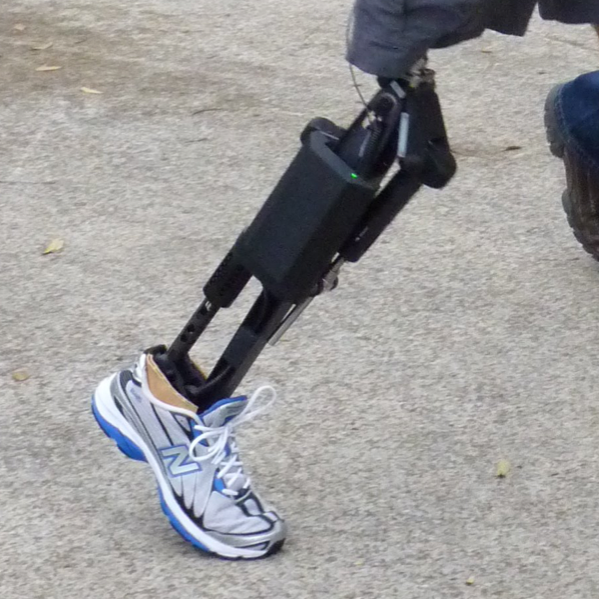
\includegraphics[height=2in]{VU_gen_1}
        \caption{Generation 1 used ball screw transmissions, \unit[200]{W}
        brushless motors, and a unidirectional parallel spring in the ankle that
        reduced motor torque requirements \citep{sup2009preliminary}.}
        \label{fig:vanderbilt_gen_1}
	\end{subfigure}
	\begin{subfigure}[t]{0.32\linewidth}
    	\centering
        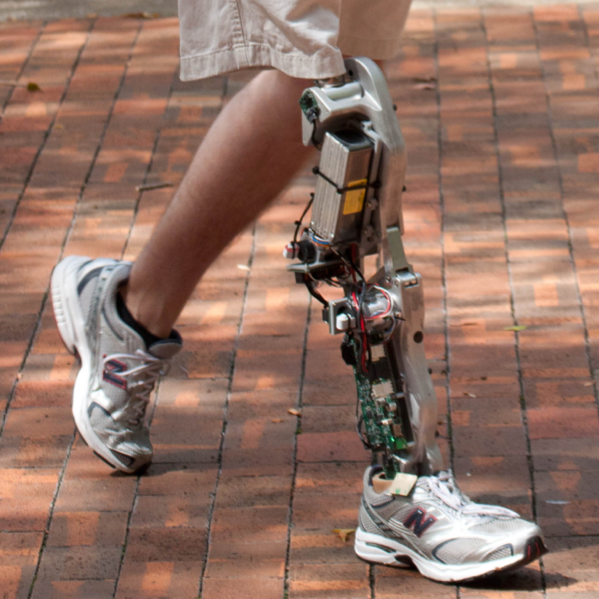
\includegraphics[height=2in]{VU_gen_2}
        \caption{Generation 2 replaced ball screws with custom gear-based
        transmission that is less noisy and more durable
        \citep{lawson2013control}.}
        \label{fig:vanderbilt_gen_2}
	\end{subfigure}
	\begin{subfigure}[t]{0.32\linewidth}
    	\centering
        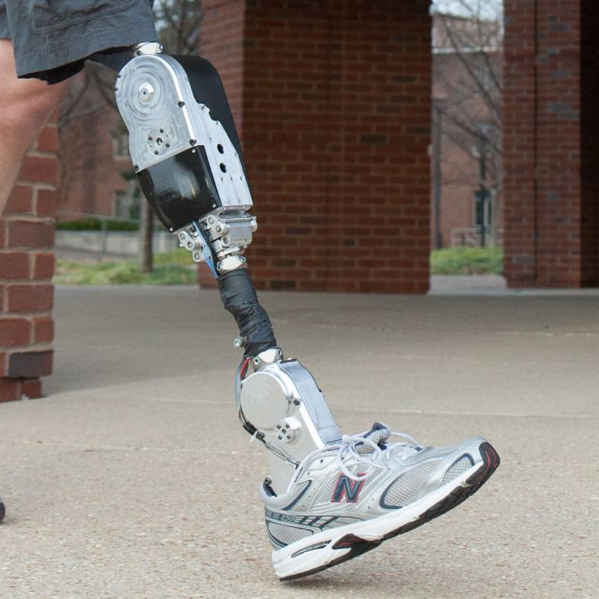
\includegraphics[height=2in]{VU_gen_3}
        \caption{Generation 3 features a modular design with separable knee and
        ankle units \citep{lawson2014robotic}.}
        \label{fig:vanderbilt_gen_3}
	\end{subfigure}
    \caption[Vanderbilt University's Robotic Transfemoral Prostheses]{Vanderbilt
    University's Robotic Transfemoral Prostheses.}
    \label{fig:vanderbilt_prostheses}
\end{figure*}

With these actuators, the knee motor can achieve the required peak torque and
peak power intermittently (\cref{tab:walking_requirements}). However, the ankle
motor may be overly stressed due to the high requirements of walking. To remedy
this, this prosthesis includes of a unidirectional parallel spring in the ankle
that reduces the required ankle motor torque. As shown in figure
\cref{fig:ankle_torque_vs_angle}, during level ground walking, a linear torsion
spring accounts for a significant portion of the ankle's torque versus angle
relationship. Therefore, incorporating a spring into the ankle offloads this
portion of the torque from the motor. The ankle motor only needs to provide the
difference between the desired output torque and the linear spring. As a result,
the spring reduces motor energy consumption, heat generation, and transmission
wear.

Further improvements resulted in two more generations of prostheses
(\cref{fig:vanderbilt_prostheses}b,c) \citep{lawson2013control,
lawson2014robotic}. These versions replaced ball screw transmissions with a
multi-stage belt/chain which improved packaging and reduced noise and wear
(Michael Goldfarb, personal communication, September 18, 2013).  With these
prostheses, researchers have extensively tested a variety of control strategies
including quasi-stiffness control \citep{sup2009preliminary, sup2011upslope,
lawson2013control, lawson2014robotic, lenzi2014speed}, EMG-based control
\citep{ha2011volitional, varol2010multiclass}, minimum jerk trajectory following
\citep{lenzi2014minimum}, and virtual constraint control
\citep{gregg2014virtual}. 

Additional prostheses in the rigid transmission category include AMPRO
\citep{zhao2016first}, and a commercially available active knee and ankle
prostheses: the Össur Power Knee and Proprio Foot. The AMPRO prosthesis features
two 374 W motors coupled to Harmonic Drive transmissions.
\citet{zhao2016first}, use this prosthesis to asses the merits of a virtual
constraint controller. The Össur Power Knee features an electric motor that can
provide torque to facilitate sit-to-stand motions, stair climbing, and active
extension and flexion during walking. The Proprio Foot also features electric
actuation that allows it to adapt to terrain and dorsiflex the ankle during
swing to help avoid trips. 

\subsubsection{Torque Control Strategies for Rigid Transmission Prostheses}
In order to achieve dynamic locomotion capabilities, it is crucial that
prosthesis designs allow for closed loop control of torques. To do this, the
control system must be able to accurately measure the torque at the joint
output. There are two main strategies for torque measurement used by prostheses
with rigid transmissions.

The first strategy is to measure the current draw of the motors windings, which
is related linearly to the motor torque. One can then multiply this measurement
by the gear ratio to obtain an estimate of the output joint torque. This is the
method used by Generations 2 and 3 of the Vanderbilt prosthesis as well as the
AMPRO prosthesis. The benefit of this method is that it utilizes existing
hardware and allows one to use high frequency current control modes of motor
drivers. However, a drawback of this method is that it measures the torque
before the transmission. Consequently, it does not account for frictional
losses, which can be difficult to model, especially for geared systems. A
strategy that deals with this problem is to install load cells in series with
the motor after the transmission, as was done on Generation 1 of the Vanderbilt
prosthesis. With this method, the closed-loop control can compensate for
frictional losses as they are included in the torque measurement. 
\begin{marginfigure}
    \centering
    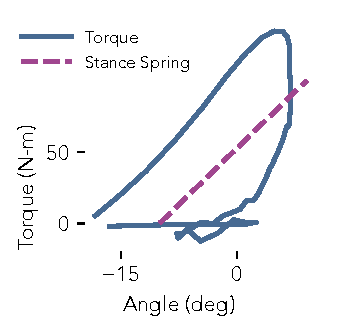
\includegraphics[width=\linewidth]{ankle_torque_vs_angle}
    \caption[Torque vs angle relationship for the ankle during level ground
    walking]{Torque vs angle relationship for the ankle during level ground
    walking. A linear spring relationship captures a significant portion of
    ankle function during stance. Data from \citet{winter2009biomechanics}
    scaled to 85 kg subject.}\label{fig:ankle_torque_vs_angle}
\end{marginfigure}

However, this method may still not address a second problem: sluggish passive
dynamics caused by reflected inertia and damping. Reflected inertia refers to
the apparent magnification of motor rotor and gearing inertia on the outside of
gearbox.  We can derive this effect through Newton's second law for the geared
motor
\begin{align}
    J_\tn{i} \ddot{\theta}_\tn{i} = \tau_\tn{i} - b_\tn{i} \dot{\theta}_\tn{i}.
\end{align}
Here, $\theta$ and its derivatives refer to angular states of the motor, $b$ is
the damping constant, $J$ is the inertia and $\tau$ is the motor torque. We use
subscript i to refer to these quantities as seen before the gear reduction, and
subscript o to refer to those quantities reflected outside of the motor.
Substituting $\theta_\tn{i} = n \theta_\tn{o}$ and $\tau_\tn{i} = \frac{1}{n}
\tau_\tn{o}$, where $n$ is the gear ratio, and multiplying through by $n$ yields
\begin{align}
    J_\tn{i} n^2 \ddot{\theta}_\tn{o} 
        &= \tau_\tn{o} - b_\tn{i} n^2 \dot{\theta}_o \\
    \implies \quad J_\tn{o} \ddot{\theta}_\tn{o} 
        &= \tau_\tn{o} - b_\tn{o} \dot{\theta}_\tn{o}.
\end{align}
These equations show that the inertia and damping of the motor rotor are
amplified by the square of the gear ratio. As prostheses may often use gear
ratios in excess of 100:1, this effect can be substantial. 

For example, \cref{tab:vanderbilt_reflec_interita} shows the calculated
reflected inertias of the Maxon Motors used in Generation 3 of the Vanderbilt
prosthesis and compares the values to the estimated inertia of the shank and
foot about the knee and the foot about its center of mass. We see that at the
knee, the reflected inertia is roughly 17\% of that of the human shank and foot.
In practice, this value is likely several times higher after including the
inertia of the encoder, bearings, and gearing. Consequently, we can estimate
that the reflected inertia may be on the order of the leg itself. At the ankle,
the reflected inertia of the rotor alone is several orders of magnitude more
than that of the foot and more than twice that of the shank and foot. When we
also consider reflected damping and friction, the dynamics of prosthesis system
may be significantly slower than assumed.
\begin{table}[t]
  \centering
  \begin{tabular}{lll}
    \toprule
    & Knee & Ankle \\
    \midrule
    rotor inertia & $\unit[0.035]{kg \cdot cm^2}$ 
        & $\unit[1.210]{kg \cdot cm^2}$\\
    gear ratio & 176:1 & 115:1 \\
    reflected inertia & $\unit[0.11]{kg \cdot m^2}$ & 
        $\unit[1.6]{kg \cdot m^2}$\\
    human inertia & $\unit[0.66]{kg \cdot m^2}$  & $\unit[0.019]{kg \cdot m^2}$\\
    percent increase & 17\% & 8400\% \\
    \bottomrule
  \end{tabular}
  \caption[Estimated reflected inertia of Generation 3 Vanderbilt
  Prosthesis]{Estimated reflected inertia at knee and ankle joints of Generation
  3 Vanderbilt Prosthesis \citep{lawson2014robotic}. Motor data taken from Maxon
  Motors Catalog\citep{maxon_flat_motor, maxon_ec4pole} Knee reflected inertia
  compared to inertia of human shank and foot about knee.  Ankle inertia
  compared to human foot about its center of mass. Human inertias estimated from
  \citet{winter2009biomechanics} for an \unit[85]{kg}, \unit[1.7]{m} tall
  person.}\label{tab:vanderbilt_reflec_interita}
\end{table}


The increase in joint impedance created by transmissions could present an issue
when attempting to execute dynamic behaviors involving impact such as running or
trip recovery. In an impact event, the impulse will move through the system at
the speed of sound through metal, roughly \unitfrac[6420]{m}{s} for aluminum
\citep{lide2004crc}. If the prosthesis is \unit[0.5]{m} long, the shock will
traverse its length in \unit[0.00008]{seconds}. This is about 10 times faster
than the typical \unit[1000]{Hz} control frequency of prosthesis control
systems, rendering closed loop torque control with load cells unresponsive. The
impact shock could cause damage to gearing and discomfort for the amputee.

%Reflected Inertia
%Vanderbilt gen 3 ankle = 1210 g*cm^2 * 115^2 in kg*m^2 = 1.6 kg*m^2
%Vanderbilt gen 3 knee = 35 g*cm^2 * 176^2 in kg*m^2 = 0.11 kg*m^2

%human leg for 1.7 85 kg = 0.6575 kg*m^2
%human foot for 1.7m 85 kg = 0.0187 kg*m^2

\subsection{Design of Dynamic Prostheses}\label{sec:back_dyn_pros}
In contrast to the rigid transmission actuation discussed in the previous
subsection, prostheses that employ series elastic actuation may be better poised
to achieve dynamic locomotion \citep{pratt1995series}. This actuation scheme
(illustrated in \cref{fig:sea_diagram}) aims to solve the torque measurement and
impedance amplification caused by transmissions by placing a spring in series
with the actuator. Measuring the deflection of the spring allows for accurate
closed-loop control of the joint torque. Moreover, the spring low-pass filters
external impulses, granting the control system more time to move the motor rotor
in response to the external load.  Due to these properties, designers have
integrated series elastic actuators into a number of bipedal robots that seek to
achieve dynamic locomotion such as M2V2 \citep{pratt2008design} and ATRIAS
\citep{grimes2013atrias}.
\begin{marginfigure}[0in]
    \centering
    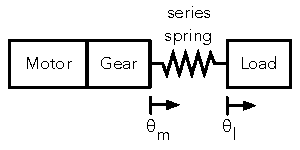
\includegraphics[width=2in]{sea_diagram}
    \caption[Series elastic actuator diagram]{Series elastic actuation inserts a
    spring between the gear output and the load (here drawn as linear actuator
    for simplicity). Torque is measured via the spring deflection, $\tau =
    k(\theta_l - \theta_m - \theta_0)$ where $\tau$ is the output joint torque,
    $k$ is the spring constant, and $\theta_l$ and $\theta_m$ are the load and
    motor positions and $\theta_0$ is the spring's rest
    length.}\label{fig:sea_diagram}
\end{marginfigure}

Series elastic actuators have found use in a variety of transtibial and
transfemoral prostheses. We can further split these applications into two
categories, those that optimize the spring stiffness for control bandwidth
subject to shock tolerance and those that optimize spring stiffness to optimize
efficiency.

\subsubsection{Springs for Bandwidth and Shock Tolerance}
Adding a spring between the gear and load introduces additional dynamics between
external torques and torques applied to the gearbox as external torques must
physically displace the load before they generate torque on the motor. This
property can improve the shock tolerance of SEA actuators over that of direct
drive motors~\citep{robinson2000design}. However, by the same token, the SEA
also introduces additional dynamics between motor torque and load torque, hence
reducing force control bandwidth. Therefore, a trade-off exists between the
compliance of the actuator and speed with which it can generate desired torques.

\citet{au2007biomechanical, au2008powered} design powered ankle prostheses with
this trade off in mind. In these publications, the authors find that using a
SEA spring soft enough to protect the ball screw transmission results in
insufficient closed loop torque control bandwidth. To overcome this shortcoming,
the authors incorporate a parallel spring into the ankle as was done for some of
the knee and ankle prostheses discussed in \cref{sec:back_rigid_trans}. Because
the parallel spring offsets the motor's torque requirements,
\citeauthor{au2008powered} find that it also improves the bandwidth of the
system from 4 Hz to 20 Hz, thereby exceeding the requirement for walking. 

\citet{caputo2013experimental} also used series elastic actuators in a robotic
prosthesis testbed. This system uses a large, \unit[1.61]{kW} offboard motor
connected to a light-weight prosthesis end-effector via a Bowden cable
transmission. The Bowden cable applies forces to one end of a fiberglass leaf
spring strain gauges measure its deflection. The author's note that the series 
springs isolate the prosthesis end effector from the motor's rotor inertia. With
this system the authors achieve a large peak output torque ($\unit[175]{N \cdot
m}$) and high bandwidth (\unit[17]{Hz}), allowing them to rapidly test the
effects of different control strategies and emulate prosthesis hardware
\citep{caputo2015informing}.

\subsubsection{Springs for energy efficiency}
Designers can also tune series elasticity in order to improve energy efficiency
by mimicking the role of tendons in the biological human leg. In the human
ankle, the Achilles tendon, which is in series with the ankle plantarflexor
muscles, stores energy throughout stance and releases it just prior to toe-off,
producing a surge of mechanical power. During this process, the ankle
plantarflexor muscles hold the proximal end of the tendon nearly stationary via
isometric contraction. This kind of length-preserving muscle contraction
consumes relatively little metabolic energy compared to concentric or
length-shortening contractions \citep{rall1984energetic}. Consequently, ankle
elasticity helps store and release energy, thereby improving metabolic cost of
walking \citep{sawicki2009pays}.

Similarly, the SPARKy prosthesis uses a \emph{Robotic Tendon} comprised of
helical springs in series with the motor to store and release energy ankle
energy during stance \citep{hitt2007sparky, bellman2008sparky,
holgate2008sparky}. Adding a series spring changes the ankle motor movement to
that required to generate desired output torque given the stiffness of the
spring and trajectory of the ankle joint\sidenote{$\theta_m = \theta_l -
\nicefrac{\tau}{k} - \theta_0$, where $\tau$ is the desired ankle torque,
$\theta_l$ is the ankle trajectory, and $k$ and $\theta_0$ are the spring
stiffness and offset}. Therefore, with a properly tuned series spring the
design reduces motor movement and thus required motor power from \unit[250]{W}
to \unit[77]{W} \citep{hitt2007sparky}.

Transfemoral prosthesis designs have also sought to use springs in the knee
joint in order to improve energy efficiency. However, these prostheses require
more sophisticated designs due to the complex behavior of the knee. Whereas a
single spring relationship explains a significant portion of ankle joint
behavior (\cref{fig:ankle_torque_vs_angle}), as shown in
\cref{fig:knee_torque_vs_angle}, the knee joint requires two springs: one for
early stance and one for pre-swing and swing. Two prostheses that tackle this
design problem are AAAKP (agonist-antagonist active knee prosthesis)
\citep{martinez2008design, martinez2011antagonistic} and the CSEA (clutchable
series elastic actuator) knee \citep{rouse2014clutchable, rouse2015design}.

The AAAKP prosthesis uses two unidirectional springs, one for extension and one
for flexion, each in series with its own actuator. With this setup,
AAAKP is able to store energy during the knee flexion phase just after heel
strike, and transfer it to a flexion spring for use during pre-swing and swing.
The prosthesis consumes just \unitfrac[5.6]{J}{stride}. However, the downside of
this design is inefficient use of actuator mass, as two electric motors are
required, one for extension and one for flexion.
\begin{marginfigure}[0in]
    \centering
    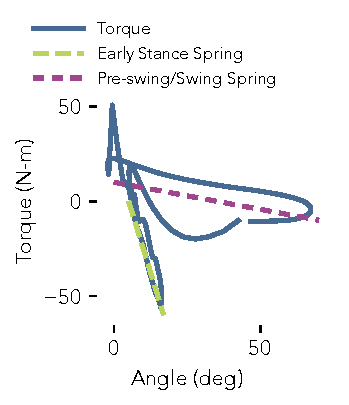
\includegraphics[width=\linewidth]{knee_torque_vs_angle}
    \caption[Torque vs angle relationship for the knee during level ground
    walking]{Torque vs angle relationship for the knee during level ground
    walking. Knee displays more complicated functionality than the ankle (see
    \cref{fig:ankle_torque_vs_angle}), with two distinct springs need to explain
    early stance and pre-swing/swing behavior. Data from
    \citet{winter2009biomechanics} scaled to 85 kg
    subject.}\label{fig:knee_torque_vs_angle}
\end{marginfigure}

A second concept is to use a series elastic actuator with a clutch on the motor
\citep{rouse2014clutchable, rouse2015design} The clutch saves energy by holding
the motor side of the series spring stationary while the spring is loaded in
early stance; no electrical energy is consumed holding the rotor in place. In
this design the spring-like behavior of the knee during swing is reproduced by
the electric motor alone unlike in the AAAKP prosthesis. Despite this, the
CSEA knee consumes less energy than the AAAKP, just \unitfrac[3.6]{J}{stride}.
Moreover, the simplified design of the CSEA has a mass of \unit[2.7]{kg} vs
\unit[3.6]{kg} for the AAAKP.

A potential drawback of SEA designs that are tuned for energy efficiency is that
they typically tune the spring stiffness to match observed quasi-stiffness
of the biological joint during a certain phase of the gait. However, this
stiffness value is not necessarily that which maximizes torque control
bandwidth. Therefore, while prostheses tuned for efficiency can consume less
energy, which is desirable for a product needing long battery life, they may
not represent the most versatile design for evaluating new control ideas or
different gait modes. 

\section{Mid-Level Control}\label{sec:back_mid_level_control}

\section{High-Level Control}\label{sec:back_high_level_control}

\section{Prosthesis Optimization}\label{sec:back_optimization}
\begin{enumerate}
    \item Zhange actor critic reinforcement learning
    \item Collins CMAES
\end{enumerate}

